\chapter{Controlling Weakly-coupled Carbon Spins}
\section{Carbon control (more of a theory chapter, change title) }
When on resonance (\cref{eq:res_dip_loc} ) the carbon rotates around on of two distinct anti-parallel axes based on the state the electron is in.
[Need some statement that puts the axis in the equator when on resonance. Look in appendix again ]
We define the

Figure of Bloch sphere whoing n0 and n1 axis.
A state starting of in 0 being rotated to +y and -y ($\pm $ x operation).
Different arrow


adf

\subsection{Carbon Ramsey experiment }



\subsection{Measuring Precession Frequencies/Carbon Ramsey experiment}
% Ramsey experiment to measure coupling strengths
% Needs relation between frequency and parralel component
% spins 1 and 4 best
Idea explain init with swap init. And from there go back to X-init. Refer to appendix for more rigorous derivation.


\begin{figure}[htbp]
    \centering
\mbox{
\Qcircuit @C=1em @R=.7em {
\lstick{\ket{0}}          & \gate{\pi/2}  & \ctrl{1}      & \qw & \multigate{1}{T}       &  \qw &\ctrl{1}          & \gate{\pi/2} &\qw          &  \meter \\
\lstick{\rho_\mathrm{m}}         & \qw              &  \gate{\pm \mathrm{x}}     & \qw& \ghost{T}        & \qw & \gate{\pm \mathrm{x}}      & \qw       &\qw&}}
    \caption{Carbon Ramsey experiment. }
    \label{fig:gate_circuit_nuclear_ramsey}
\end{figure}

\begin{figure}[htbp]
    \centering
\mbox{
\Qcircuit @C=1em @R=.7em {
\lstick{\ket{0}_e}                        & \gate{\mathrm{y}}  & \ctrl{1}       & \gate{x} &\qw          &  \meter &\qw\\
\lstick{\rho_\mathrm{m}}         & \qw              &  \gate{\pm \mathrm{x}}     & \qw    & \qw   & \qw       &\qw&}}
    \caption{MBI-based initialization into $\pm \ket{\mathrm{X}}$. Initializes the carbon into $\ket{X}_C $ when $\ket{0}_e$ is measured and into $\ket{-X}_C $ when $\ket{1}_e$ is measured for the electron.}
    \label{fig:gate_circuit_mbi_x-init}
\end{figure}

\begin{figure}[htbp]
    \centering
\mbox{
\Qcircuit @C=1em @R=.7em {
\lstick{\ket{0}_e} & \gate{\mathrm{y}}  & \ctrl{1} & \gate{x} &\ctrl{1} &  \meter &\qw\\
\lstick{\rho_\mathrm{m}}& \qw&  \gate{\pm \mathrm{x}}     & \qw    & \gate{\pm \mathrm{y}}    & \qw       &\qw&}}
    \caption{MBI-swap initialization into $\pm \ket{\mathrm{0}}$. Initializes the carbon into $\ket{0}_C $ when $\ket{0}_e$ is measured and into $\ket{1}_C $ when $\ket{1}_e$ is measured for the electron.}
    \label{fig:gate_circuit_mbi_swap-init}
\end{figure}


\begin{figure}[htbp]
    \centering
\mbox{
\Qcircuit @C=1em @R=.7em {
\lstick{\ket{0}_e} & \gate{\mathrm{y}}  & \ctrl{1} &  \ctrl{2} & \gate{y}  &  \meter &\qw\\
\lstick{\ket{0}_{C1}} & \qw&  \gate{\pm \mathrm{x}}  &\qw  & \qw       &\qw&\qw& \\
\lstick{\ket{0}_{C2}}& \qw& \qw  & \gate{\pm \mathrm{x}}    & \qw      &\qw&\qw&}}
    \caption{XX-parity-measurement}
    \label{fig:gate_circuit_XX-parity-measurement}
\end{figure}

\begin{figure}[htbp]
    \centering
\mbox{
\Qcircuit @C=1em @R=.7em {
\lstick{\ket{0}_e} & \gate{\mathrm{y}}  & \ctrl{1} &  \ctrl{2} & \gate{\mathrm{y}}  & \ctrl{1} &  \ctrl{2} &  \meter &\qw\\
\lstick{\ket{0}_{C1}} & \qw&  \gate{\pm \mathrm{x}}  &\qw  &\qw  & \gate{\pm \mathrm{x}} & \qw   &\qw&\qw& \\
\lstick{\ket{0}_{C2}}& \qw& \qw  & \gate{\pm \mathrm{x}}    & \qw    &\qw& \gate{\pm \mathrm{x}}    & \qw &\qw&}}
    \caption{General parity RO}
    \label{fig:gate_circuit_general_Parity_RO}
\end{figure}


\begin{figure}[htbp]
    \begin{subfigure}[t]{0.49\textwidth}\centering
    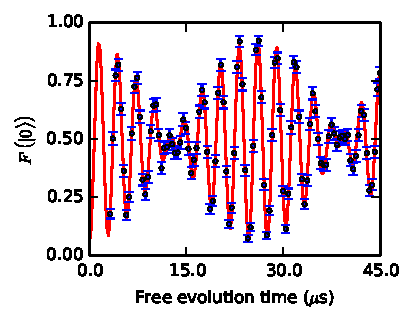
\includegraphics{Img/CarbonRamsey_C1.pdf}
    \caption{Nuclear Ramsey of Carbon 1} \label{fig:CR_C1}
    \end{subfigure}
    \begin{subfigure}[t]{0.49\textwidth}\centering
        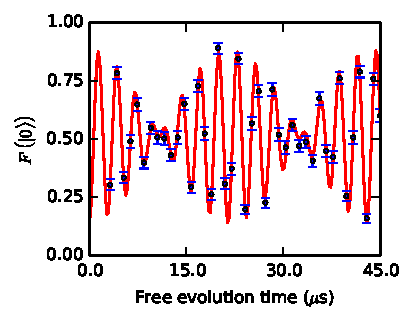
\includegraphics{Img/CarbonRamsey_C4.pdf}
        \caption{Nuclear Ramsey of Carbon 4}
        \label{fig:CR_C4}
    \end{subfigure}
    \caption{Nuclear Ramsey experiment wit}
\end{figure}



\section{Controlling weakly coupled carbons trough the electronic spin}
% Section containing theory (Gate circuits) on how to initialize and readout carbons

Explain how carbon control works in theory.
Explain how a conditional and unconditional gate can be performed.
Explain initialization on gate level, refer to appendix for calculations.
Explain Readout.

\subsection{Initialized Carbon Ramsey}


\section{Carbon Initialization \& Readout}
% TODO_MAR: Discuss naming of sec: Carbon Init&RO and Carbon Tomo
%  Section containing experimental results (Tomographies)
%  Should emphasize difficulty in seperating initialization and RO fidelity, what is not working? Is it working?
Show results that demonstrate carbon control.



